\section{Background}

\Egglog is designed as a Datalog variant
 with extensions that make it subsume \eqsat.
% \of{I think this undersells it as "just datalog with eqsat"}
This section will introduce both Datalog and \eqsat
 in their own terms,
 while \autoref{sec:overview}
 will show how they both fit within the \egglog framework.

\subsection{Datalog}
\label{sec:datalog}

\autoref{fig:datalog-tc}
 shows a Datalog program to compute the transitive closure of a graph.
Datalog is a recursive database query language that
 represents data as \emph{relations}.
Each relation is a set of tuples, and all tuples in 
  the same relation share the same arity.
A Datalog program consists of a set of \emph{rules}.
Each rule is a \emph{conjunctive query} of the form
\(
  Q(\mathbf{x}) \ngets 
  R_1(\mathbf{x}_1), R_2(\mathbf{x}_2), \ldots, R_n(\mathbf{x}_n)
\)
where each $\mathbf{x}$ and $\mathbf{x}_i$ is a tuple of variables or constants. 
The atom $Q(\mathbf{x})$ is called the \emph{head} of the rule, 
  and the atoms $R_i(\mathbf{x}_i)$ comprise the \emph{body}.
The body binds variables to be used in the head to create new facts;
 all variables in the head must appear in the body.
Specifically, running a rule adds the following facts:
\(
  \{
    Q(\mathbf{x}[\sigma]) \mid
    \bigwedge_i \mathbf{x}_i[\sigma] \in R_i
  \}
\),
where $\sigma$ is a substitution 
 that maps all the variables in the rule to constants.
In other words,
 querying the body creates substitutions such that
 every substituted body atom is in the database;
 these substitutions are then applied to the head to create new facts.
% Note in a rule with an empty body, $Q(\mathbf{x}) \ngets.$, 
%   also written as $Q(\mathbf{x}).$,
%   $\mathbf{x}$ may only contain constants, 
%   and the rule assigns to $Q$ the set $\set{\mathbf{x}}$.

% The rule assigns to $Q$ the set $\setof{t}{t_1 \in R_1, t_2 \in R_2, \ldots, t_n \in R_n}$, 
%   such that substituting $t$ for $\mathbf{x}$ and $t_i$ for $\mathbf{x}_i$
%   results in a consistent substituion\footnote{A substituion is consistent 
%   if it maps every constant to itself, and every variable to a unique constant.}.
% Each rule can be seen as a function from the relations in the body
%   to the head relation $Q$. 
% The set of all rules in a Datalog program therefore defines 
%   a function from \emph{all} body atoms to all head atoms;
%   if two rules share the same head atom, 
%   then we apply each rule and take the union of the results.
Each rule can be seen as a function 
 from the current database to a new database that includes
 the facts created by the rule;
 call this function $T_r$ for some rule $r$.
The set of all rules $r$ in a Datalog program $p$ 
 therefore defines a function $T_p$ 
 from the current database to a new database: 
 $T_p(\mathsf{DB}) = \bigcup_{r \in p} T_r(\mathsf{DB})$.
This function is called the immediate consequence operator (ICO) of the program,
  which we denote $T_p$.
To run a Datalog program, we start with an empty database and
 repeatedly apply $T_p$ until the database stops changing.
A fundamental result in Datalog is that every program terminates, 
  and the final result is the least fixpoint of $T_p$~\citep{alice-book}.

% \pz{I feel like this description is missing that the database is accumulating.
% It needs $T_p(DB) = DB \cup \bigcup T_r$ or it needs a union over every timestep.
% }
% \rw{We have a rule for each fact, so you don't need to explictly accumulate. This is the standard.}

\begin{figure}
\begin{subfigure}[b]{0.4\linewidth}
\begin{align*}
E(1, 2)&. \\
E(2, 3)&. \\
E(3, 4)&. \\
TC(x, y) & \ngets E(x, y). \\
TC(x, y) & \ngets TC(x, z), E(z, y).
\end{align*}
\caption{
  Transitive closure in Datalog.
  Facts (e.g. $E(1, 2)$) are given as rules without bodies.
}\label{fig:datalog-tc-code}
\end{subfigure}
\hfill
\begin{subfigure}[b]{0.55\linewidth}
\begin{tabular}{lll}
    iter\# & E & TC \\
    \hline 
    0 & $\emptyset$ & $\emptyset$ \\
    1 & $\set{(1,2),(2,3),(3,4)}$ & $\emptyset$ \\
    2 & $\set{\ldots}$ & $\set{(1,2),(2,3),(3,4)}$ \\
    3 & $\set{\ldots}$ & $\set{\ldots, (1,3),(2,4)}$ \\
    4 & $\set{\ldots}$ & $\set{\ldots, (1,4)}$ \\
\end{tabular}
\caption{
  Execution trace of transitive closure. 
  ``$\ldots$'' includes tuples from the cell directly above.
}
\label{fig:datalog-tc-exec}
\end{subfigure}
\caption{
  Transitive closure is the classic Datalog example.
  It iteratively computes the transitive closure ($TC$) 
  of an edge relation $E$
  by applying the rules in \autoref{fig:datalog-tc-code}.
}\label{fig:datalog-tc}
\end{figure}


% As an example, consider the Datalog program in \autoref{fig:datalog-tc}.
% \autoref{fig:datalog-tc-exec} traces the execution of the program,
%   showing the content of each relation after each application of $T_p$.
% Note that each relation retains all tuples from the previous step.
% This is because $T_p$ is \emph{monotonic}, a crucial property for the fixpoint semantics
%   described above.
% \yzinline{%
%   The property of retaining all tuples and monotonicity 
% does not necessarily imply each other. 
% The former is called inflationary. \Egglog's ICO is inflationary, but not necessarily monotonic.
% See \url{https://en.wikipedia.org/wiki/Bourbaki\%E2\%80\%93Witt\_theorem}
% }
% \rw{Inflationary doesn't imply monotone, but if $f$ is monotone and $f(\bot) \geq \bot$. 
% Monotonicity is also necessary for the \emph{least} fixpoint. 
% I think it is important to be precise here, and clarify \Egglog's semantics later.}

Datalog became popular in programming languages research 
  as a declarative language for specifying large-scale program analyses
  such as points-to analyses~\cite{doop-datalog}.
In order to support abstract interpretation-style analyses,
  researchers have extended Datalog to work over lattices.
% To understand this extension, 
%   consider each relation as a function from tuples to booleans:
%   $R(t) = \mathsf{true}$ iff $t \in R$ and false otherwise.
% \pz{This is good and simple and yet not how I think about it. It isn't a function to Bool in my head.
% It's either partial functions to unit, or functions to the True/Unknown lattice.
% Does making this point nicely directly lead to the lattice datalog concept?
% }
% \rw{I call Uknown ``false''}
In the lattice semantics,
 a relation is viewed as a function from tuples to a lattice,
We then generalize Datalog rules to be over functions:
\(
  Q(\mathbf{x}) \!\mapsto\! x
  \ngets 
  R_1(\mathbf{x_1}) \!\mapsto\! x_1, 
  \cdots, 
  R_n(\mathbf{x_n})\!\mapsto\! x_n
\).
% \(
%   Q(\mathbf{x}) 
%   = \bigvee_{\mathbf{x}_\text{free}} R_1(\mathbf{x_1}) \wedge R_2(\mathbf{x_2}) \wedge \cdots \wedge R_n(\mathbf{x_n})
% \)
% where $\mathbf{x}_\text{free}$ is the set of variables in the body that do not appear in the head,
%  and each $x\in \mathbf{x}_\text{free}$ ranges over the entire domain.
% We can 
%  generalize this to any semi-lattice
%  by replacing $\vee$ and $\wedge$
%  with 
%  $\sqcup$ (lattice join) and some function $\times$ 
%  that is monotone according to the lattice's ordering.
% We then interpret a rule as 
% \(
%     Q(\mathbf{x}) = 
%     \bigsqcup_{\mathbf{x}_\text{free}} R_1(\mathbf{x_1}) \times R_2(\mathbf{x_2}) \times \cdots \times R_n(\mathbf{x_n}) 
% \)
% where $\times$ is some function that is monotone according to the ordering induced by the lattice.
% Using the boolean lattice yields
%  classic Datalog as defined above,
%  but others allow for richer computations.
% For example, 
%  with the semi-lattice over $\mathbb{N}$ where $(\sqcup, \times) \defeq (\min, +)$,
%  the last two rules in \autoref{fig:datalog-tc}
%  compute the shortest distance between any pair of vertices.
The value of $Q$ on input $\mathbf{x}$ is 
 the supremum of valid $x$s producible by the body, i.e.,
% \[
%   \bigsqcup_{\substack{
%     \mathbf{x}_\text{free}\\
%     R_1(\mathbf{x_1})=x_1\\
%     \ldots\\
%     R_n(\mathbf{x_n})=x_n
%   }} x
% \]
$Q(\mathbf{x})=
  \bigsqcup
  % \left
  \{
    x \mid
    \bigvee_{\mathbf{x}_\text{free}}
    R_1(\mathbf{x_1})=x_1 \land
    \ldots\land
    R_n(\mathbf{x_n})=x_n
  % \right
  \}
$
where $\mathbf{x}_\text{free}$ is the set of variables in the body 
 that do not appear in the head and $\sqcup$ is 
 a lattice join (i.e., supremum) operator.
\Egglog's support for lattices
 is motivated by other 
 modern Datalog implementations~\cite{datalogo,ascent,flix}
 that support this extension.
% \mw{cite flix}
% \pz{does a mention of semiring semantics fit here or 
% just confuses the picture?}
% \rw{We can cite it, but semiring and flix are essentially the same for what we care.}

\subsection{Equality Saturation}

\begin{figure}
    \begin{subfigure}[t]{0.30\linewidth}
        \centering
        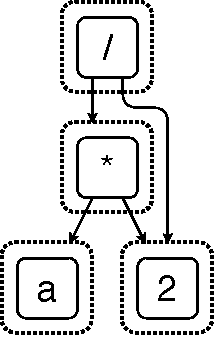
\includegraphics[scale=0.5]{figs/overview1.pdf}
        \caption{\Egraph represents $(a\times 2)/2$.}
    \end{subfigure}
    \hfill
    \begin{subfigure}[t]{0.30\linewidth}
        \centering
        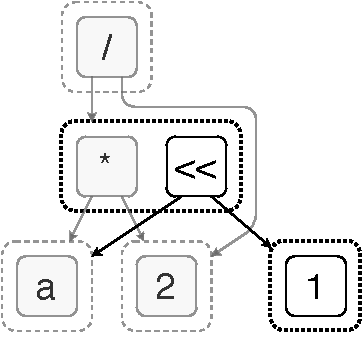
\includegraphics[scale=0.5]{figs/overview2.pdf}
        \caption{Rewrite \mbox{$x\times 2\rightarrow x\ll 1$}.}
    \end{subfigure}
    \hfill
    \begin{subfigure}[t]{0.30\linewidth}
        \centering
        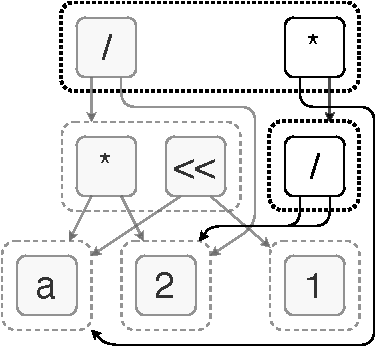
\includegraphics[scale=0.5]{figs/overview3.pdf}
        \caption{Rewrite $(x\times y)/z\rightarrow x\times(y/z)$.}
    \end{subfigure}
    \caption{Applying rewrites over an example \egraph (figures from \citet{egg}). 
    A solid box denotes an \enode, and a dotted box denotes an \eclass.
    \Enodes consist of a function symbol and children \eclasses, 
    and \eclasses contain a set of \enodes.}
    \label{fig:egraphs}
\end{figure}

% Term rewriting is at the core of modern program optimizers.
% In term rewriting,
%  a term is rewritten according to a series of rewrite steps to its final form.
% However, a key challenge to program optimization via term rewriting is that,
%  applying one rule may disable another.
% For example, rewriting $(a\times 2)/ 2$ to $(a\ll 1)/2$ may prevent future rewrites 
%  to cancel out $2/2$.
% This is known in the compiler literature as the phase ordering problem.

Traditional term rewriting applies one rule at a time 
 and forgets the original term after each step, 
 so it is sensitive to the ordering of the rewrites.
For example, rewriting $(a\times 2)/ 2$ to $(a\ll 1)/2$ 
 is locally good, but it prevents future opportunities to cancel out $2/2$.
Equality saturation (\eqsat)~\cite{eqsat}
 is a technique to mitigate this
 phase-ordering problem.
\eqsat fires all the rules in each iteration 
 and keeps both original and rewritten terms in a special data structure called the \egraph.
An \egraph~\cite{nelson} is a compact data structure 
 that represents large sets of terms efficiently.
An \egraph is a set of \emph{\eclasses}, 
 and each \eclass is a set of equivalent \emph{\enodes}.
An \enode is function symbol with children \eclasses (not \enodes).

An \egraph can compactly represent 
 an exponential number of terms compared to the size of the \egraph.
We say an \egraph \emph{represents} a term $t$
 if any of its \eclasses represents $t$,
 and an \eclass represents $t$ 
 if any \enode in the \eclass represents it.
An \enode $t = f(c_1,\ldots, c_n)$
%  with function symbol $f$ and 
%  children \eclasses $c_1,\ldots,c_n$
 represents a term $f(t_1,\ldots, t_n)$ 
 if each $c_i$ represents $t_i$.
An \egraph induces an equivalence relation 
 over terms: two terms are considered equivalent 
 if they are represented by the same \eclass.
This equivalence relation is also congruent: 
 if an \egraph represents two terms
 $a = f(a_1,\ldots, a_n)$ and $b = f(b_1,\ldots, b_n)$
 such that \egraph shows $a_i \equiv b_i$,
 then the \egraph can also show $a \equiv b$.%
\footnote{
  In \egraph implementations that canonicalize \enodes,
  congruence amounts to deduplication of \enodes
  since nodes $a$ and $b$ would canonicalize to identical \enodes.
}

% Compared to the classical tree representation of terms,
%  a node in an \egraph can have many alternative children \enodes.
% We say an \egraph \emph{represents} a term $t$
%  if it can be found in the \egraph 
%  by picking appropriate \enodes in each \eclass in a subtree:

% More formally, we say an \egraph represents $t$
%  if any of its \eclasses represents $t$,
%  and an \eclass represents $t$ 
%  if any \enode in the \eclass represents it.
% An \enode $f(c_1,\ldots, c_n)$ with function symbol $f$ and 
%  children \eclasses $c_1,\ldots,c_n$
%  represents a term $f(t_1,\ldots, t_n)$ 
%  if they share the same function symbol $f$ and $c_i$ represents $t_i$ for $i=1,\ldots, n$.
% Moreover, an \egraph represents an equivalence relation 
%  over the terms it represents: two terms are equivalent 
%  if they share the same root \eclass.

\autoref{fig:egraphs} shows an example \egraph 
 and two rule applications.
We start with the initial \egraph representing only term $(a\times 2)/2$.
To apply a rewrite rule $x\times 2\rightarrow x\ll 1$,
 we first search for matches of left-hand patterns 
 using a procedure called \emph{\ematching} (pattern matching modulo equality).
This produces substitutions (in this case, only one: $\set{x \mapsto a}$)
 that we then we apply to right-hand side pattern.
Each resulting term (e.g., $a \times 2$) is finally merged 
 into the \eclass that the left-hand side pattern matched.

% A key property to ensure the compactness in \egraphs is congruence.
% \Egraphs typically represent a congruence relation over terms.
% Congruence means that 
%  \mbox{$(\forall_i a_i = b_i) \rightarrow f(a_1,\ldots, a_n) = f(b_1,\ldots, b_n)$}.
% Congruence means that two \enodes $f(c_1,\ldots, c_n)$ and $f(c'_1, \ldots, c'_n)$
%  are in the same \eclass if $c_i$ and $c'_i$ are in the same \eclass for $i=1\ldots n$.
% This ensures that any term represented in an \egraph will 
%  only be contained in one \eclass and therefore has only one occurrence.
% This property maximizes the sharing within \egraphs 
%  and sets \egraphs apart from other similar data structures for program space representations 
%  like finite tree automata and version space algebras.
% Moreover, it guarantees the correctness of the equivalence closure
%  an \egraph represents: if two \eclasses ever represent the same term,
%  this means that terms represented by the the two \eclasses are all equivalent 
%  because of transitivity of equivalence, and therefore the two \eclasses
%  should be merged as one.

\paragraph{Extensions}
Standard \eqsat is purely syntactic.
In some cases, 
 this prevents users from writing sound rewrites.
For example,
 the rewrite $\sqrt{x^2}\rightarrow x$ 
 is sound iff $x$ is non-negative,
 but proving this requires semantic analyses.
A recent technique called \eclass analyses~\cite{egg}
 allows for semantic analyses in \eqsat.
An \eclass analysis associates every \eclass in an \egraph 
 with a semi-lattice value that is a semantic abstraction of the term.
During the \eqsat algorithm,
 the lattice data are propagated
 from children to parents \eclasses, and merged via lattice joins.
For example, 
 an analysis could track the lower bounds of \eclasses,
 which are initially $-\infty$ and increase over time
 as new terms are represented in these \eclasses via rewrites.
In \egg,
 the most popular \eqsat toolchain,
 \eclass analyses are currently limited.
An \egraph can 
 only have a single \eclass analysis,
 it can only propagate information \emph{upwards} from children to parents,
 and it requires writing low-level code in the host programming language (Rust in \egg's case).
%  \of{Could we elaborate on the limitations and why it's fundamentally hard? As in, why can't two analysis depend on each other?
%  I think it's because rebuilding is limited. 
% YZ: this may be too long to explain. Comment out for now.}


% The standard equality saturation is not sufficient 
%  for many practical applications,
%  so people use several extensions to equality saturation in practice.
% For example,
%  sometimes purely syntactic rules 
%  are not capable of expressing sound rewrites.
% The rewrite rule $\sqrt{x^2}\rightarrow x$ 
%  is only sound if and only if $x$ is {\it always} non-negative.
% But to guarantee this property requires analyses beyond syntactic.
% A technique for semantic analyses in equality saturation is called \eclass analyses.
% An \eclass analysis associates every \eclass in an \egraph 
%  with a (semi-)lattice value that is a semantic abstraction of the term.
% During the execution of equality saturation,
%  the lattice data are grown via propagations 
%  from children to parents \eclasses and merged via lattice joins.
% For example, 
%  an analysis may track the lower bounds of \eclasses,
%  which are initially $-\infty$ and increases over time
%  as new terms are represented in these \eclasses via rewrites.
% After a analysis is defined,
%  a rewrite applier (i.e., the right-hand side of a rewrite rule) 
%  can add the side condition that requires 
%  the analysis data to satisfy certain conditions 
%  (e.g., the lower bound is greater than zero).
% Contrary to the rewrite rules themselves,
%  both the \eclass analyses and the conditional applier
%  are typically written in a host language like Rust.
% \yz{visual demos for \eclass analyses?}
% \yz{mention the limitation of \eclass analyses? e.g., single analysis, not composable.}

\def\matmul{\mathit{matmul}}
\def\split{\mathit{split}}
\def\concat{\mathit{concat}} 
Multi-patterns are another commonly used extension to \ematching (and thus \eqsat).
Typically, \ematching only supports patterns matching a single term each.
A multi-pattern is a set of multiple patterns to be matched simultaneously.
For example, TenSat~\citep{tensat} is 
 an equality saturation based tensor graph optimizer
 that uses rewrite rules to share matrix multiplications.
% \yzinline{TODO: is there a more precise term than ``share matrix multiplicatins''?}
It matches patterns $e_1 = \matmul(M_1,M_2)$ and $e_2 = \matmul(M_1,M_3)$ 
 simultaneously, 
 and then creates the expression $e_3 = \matmul(M_1,\concat(M_2,M_3))$
 and merges $e_1$ with $\split_1(e_3)$ and $e_2$ with $\split_2(e_3)$.
Previous works have developed algorithms for multi-patterns~\citep{tensat, ematching},
 but they are suboptimal and complex.

Relational \ematching~\citep{relational-ematching} 
 is a recent technique to improve \ematching performance, 
 including on multi-patterns,
 by reducing it to a relational query.
%  is a promising recent work 
%  on improving the matching procedure in \egraphs, 
%  which is usually a performance bottleneck.
% It views an \egraph as a relational database,
%  and matching patterns come out naturally as relational queries.
% This both provides asymptotic speedups for a large class of queries 
%  and simplifies the implementations of both standard \ematching 
%  and multi-patterns.
However, relational \ematching suffers from the ``dual representation'' problem.
An equality saturation engine has to 
 switch back and forth between the \egraphs and 
 the relational database representations.
This can sometimes take a significant amount of the run time,
 reducing the benefits of this approach.
% Currently, 
%  there is no real-world equality saturation system that uses relational \ematching
%  that we are aware of.
Relational \ematching hints 
 at the fundamental connection between \egraphs and relational databases,
 but it only applies the insights to \ematching.
We further exploit the connection in \egglog,
 building a Datalog-inspired system that
 captures the entire \eqsat algorithm and goes beyond.

% To achieve this, we need to process all the abstractions in equality saturation relationally
% % The key to our approach is that we draw theories from the database literature
% %  and apply them to the relational representation of \egraphs.
% % In fact, database theories have already developed 
% %  all the right relational abstractions we need.
% Our key insight is that database theories have already developed all the right relational abstractions we need.
% For example, equality saturation and Datalog are similar in many aspects:
%  both systems start from the initial facts, 
%  iteratively match on known facts,
%  and non-destructively derive new facts based on matched results.
% % In a Datalog-like language, multi-patterns are supported ``for free'',
% %  since the body of a rule can naturally contain multiple atoms.
% Moreover,
%  the congruence property of \egraphs can be simply expressed 
%  as a functional dependency in the relational databases.
% \Eclass analyses, on the other hand,
%  are exactly captured by the lattice semantics of Datalog~\citep{flix}.
